%%% Содержимое слайдов

\frame[plain]{\titlepage} % Титульный слайд

%-------------------------------------------------------------------------------

\section{Стандарты безопасности}

\begin{frame}
\frametitle{\insertsection}
\framesubtitle{Но пока нет, пусть повисит график мунина}

\begin{itemize}
    \item Cloud Security Alliance (CSA)
    \item Internet Engineering Task Force (IETF)
    \item National Institute of Standards and Technology (NIST)
    \item International Telecommunications Union (ITU)
    \item Open Cloud Consortium (OCC)
    \item Object Management Group (OMG)
    \item Open Data Center Alliance (ODCA)
\end{itemize}
\end{frame}

%-------------------------------------------------------------------------------

\section{Угрозы безопасности}

\begin{frame}
\frametitle{\insertsection}
\framesubtitle{Но пока нет, пусть повисит график мунина}

\begin{itemize}
    \item утечка данных
    \item компрометация учетных записей и обход аутентификации
    \item взлом интерфейсов и API
    \item уязвимость используемых систем
    \item кража учетных записей
    \item инсайдеры-злоумышленники
    \item целевые кибератаки
    \item перманентная потеря данных
    \item недостаточная осведомленность
    \item злоупотребление облачными сервисами
    \item DDoS-атаки
    \item совместные технологии, общие риски
\end{itemize}
\end{frame}

% Расписать кратко по нескольким пунктам

%-------------------------------------------------------------------------------

\section{Борьба с проблемами}

\begin{frame}
\frametitle{\insertsection}
\framesubtitle{Но пока нет, пусть повисит график мунина}

\begin{itemize}
    \item многофакторная аутентификация (2FA) и стойкое шифрование (TLS)
    \item использование одноразовых паролей, токенов, USB-ключей, смарт-карт
    \item контроль доступа, шифрование API
    \item периодические пентестинги, аудиты безопасности
    \item регулярное сканирование на наличие уязвимостией
    \item тщательный мониторинг, аудит и логирование
    \item резервное копирование, репликация
    \item резервирование сетевых каналов и сегментация сети
\end{itemize}
\end{frame}

%-------------------------------------------------------------------------------

\section{Что хочу решать я}

\begin{frame}
\frametitle{\insertsection}
\framesubtitle{Но пока нет, пусть повисит график мунина}

\begin{itemize}
    \item структурирование всей имеющейся информации
    \item системный анализ информации
    \item с помощью метода анализа иерархий выбор альтернатив на основе набора критериев
    \item практическое применение имеющейся информации
    \item анализ наиболее опасных уязвимостей и методы взлома
    \item использование уязвимости на проде
    \item наискорейшие методы обнаружения уязвимостей в ПО (vulncontrol) и их закрытие (kernelcare)
\end{itemize}
\end{frame}

%-------------------------------------------------------------------------------

\section{Системный анализ}

\begin{frame}
\frametitle{\insertsection}
\framesubtitle{1 2 3}

\begin{itemize}
    \item цель проектирования - разработка системы безопасности облачной среды
    \item выделение входных и выходных данных
    \item выделение функций
    \item выделение подсистем: аутентификации, авторизации, сетевой защиты, проверки целостности данных
    \item модульность системы
    \item детализация функций
    \item соблюдение принципа иерархии
    \item сочетание централизации и децентрализации
    \item возможность расширения системы
    \item учет неопределенностей и случайностей
\end{itemize}
\end{frame}

%-------------------------------------------------------------------------------

\section{Вариантный анализ}

\begin{frame}
\frametitle{\insertsection}
\framesubtitle{Пример --- выбор гипервизора}
Альтернативы:
\begin{itemize}
    \item KVM (альтернатива А)
    \item Hyper-V (альтернатива Б)
    \item VMware vSphere (альтернатива В)
\end{itemize}

Критерии, по которым выбирается тот, или иной алгоритм:
\begin{itemize}
    \item цена (А1)
    \item масштабируемость (А2)
    \item отказоустойчивость (А3)
    \item интерфейсы управления (А4)
\end{itemize}

\begin{table}[H]
    \begin{tabular}{|l|l|l|l|l|l|}
      \hline \multicolumn{2}{|c|}{Критерии} & A1 & A2 & A3 & A4 \\
      \hline A1 & Цена & 1 & 1/5 & 1/7 & 3 \\
      \hline A2 & Масштабируемость & 5 & 1 & 1/5 & 7 \\
      \hline A3 & Отказоустойчивость & 7 & 5 & 1 & 8 \\
      \hline A4 & Интерфейсы управления & 1/3 & 1/7 & 1/8 & 1 \\
      \hline
    \end{tabular}
\end{table}

\begin{itemize}
    \item цель проектирования - разработка системы безопасности облачной среды
    \item выделение входных и выходных данных
    \item выделение функций
\end{itemize}
\end{frame}

%-------------------------------------------------------------------------------

\section{Критические уязвимости 2016}

\begin{frame}
\frametitle{\insertsection}
\framesubtitle{1 2 3}

\begin{table}[H]
    \begin{tabular}{|l|l|p{4cm}|l|}
        \hline CVE ID & CVSS & Тип уязвимости & ПО \\
        \hline CVE-2016-5195 & 7.2 & Получение привилегий & Linux Kernel \\
        \hline CVE-2016-6258 & 7.2 & Получение привилегий & Xen \\
        \hline CVE-2016-5696 & 5.8 & Получение данных & Linux Kernel \\
        \hline CVE-2016-3710 & 7.2 & Запуск кода & QEMU \\
        \hline CVE-2016-8655 & 7.2 & Получение привилегий, DoS & Linux Kernel \\
        \hline CVE-2016-4997 & 7.2 & Получение привилегий, DoS, доступ к памяти & Linux Kernel \\
        \hline CVE-2016-4484 & 7.2 & Получение привилегий & CryptSetup \\
        \hline CVE-2016-6309 & 10.0 & DoS, запуск кода & OpenSSL\\
        \hline
    \end{tabular}
\end{table}
\end{frame}

%-------------------------------------------------------------------------------

\section{Эксплуатация CVE-2016-5195}

\begin{frame}
\frametitle{\insertsection}
\framesubtitle{Dirty COW}

%\begin{verbatim}
{\small \texttt{\$ id \\
{\color{green} uid=1000(dcow)} gid=1000(dcow) groups=1000(dcow) \\
\$ g++ dcow.cpp -std=c++11 -pthread -o dcow -lutil}}

\vspace{\baselineskip}

{\small \texttt{\$ ./dcow \\
Running ... \\
Received su prompt (Password: ) \\
Root password is: dirtyCowFun \\
Enjoy! :-)}}

\vspace{\baselineskip}

{\small \texttt{\$ su root \\
Password: dirtyCowFun \\
\# id \\
{\color{red} uid=0(root)} gid=0(root) groups=0(root)
}}
\end{frame}

%-------------------------------------------------------------------------------

\section{Vulncontrol}

\begin{frame}
\frametitle{\insertsection}
\framesubtitle{1 2 3}

{\scriptsize \texttt{\$ ./vulncontrol.py −d 2017−02−18 −m 5 \\
CVE−2017−6074 9.3 http://www.cvedetails.com/cve/CVE−2017−6074/ \\
CVE−2017−6001 7.6 http://www.cvedetails.com/cve/CVE−2017−6001/ \\
CVE−2017−5986 7.1 http://www.cvedetails.com/cve/CVE−2017−5986/ \\
Telegram alert not sent
}}

\begin{figure}[h]
    \center
    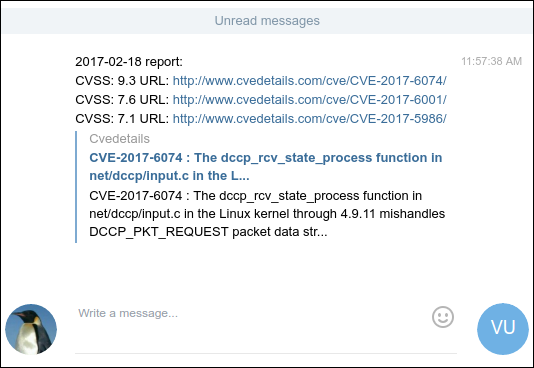
\includegraphics[width=0.65\linewidth]{tscreen}
\end{figure}
\end{frame}

%-------------------------------------------------------------------------------

\iffalse
максимум 10 слайдов
по 1 минуте на слайд
картинки, схемы, таблицы, примеры кода, списки, скриншоты

обзор источников
системный анализ
вариантный анализ
безопасность облачных вычислений
экспериментальные исследования
- крит. уязвимости
- эксплуатация dirty cow
- vulncontrol
анализ результатов

1. описать актуальность исследования
2. описать текущие проблемы в облаках
3. как эти проблемы решаются
4. какие проблемы не решаются
5. что я сделал для решения проблем
...
\fi